\iffalse
This file is protected by Copyright. Please refer to the COPYRIGHT file
distributed with this source distribution.

This file is part of OpenCPI <http://www.opencpi.org>

OpenCPI is free software: you can redistribute it and/or modify it under the
terms of the GNU Lesser General Public License as published by the Free Software
Foundation, either version 3 of the License, or (at your option) any later
version.

OpenCPI is distributed in the hope that it will be useful, but WITHOUT ANY
WARRANTY; without even the implied warranty of MERCHANTABILITY or FITNESS FOR A
PARTICULAR PURPOSE. See the GNU Lesser General Public License for more details.

You should have received a copy of the GNU Lesser General Public License along
with this program. If not, see <http://www.gnu.org/licenses/>.
\fi
%----------------------------------------------------------------------------------------
% Update the docTitle and docVersion per document
%----------------------------------------------------------------------------------------
\def\docTitle{Generic RF Interface Guide}
\def\docVersion{1.4}
%----------------------------------------------------------------------------------------
\documentclass{article}
\iffalse
This file is protected by Copyright. Please refer to the COPYRIGHT file
distributed with this source distribution.

This file is part of OpenCPI <http://www.opencpi.org>

OpenCPI is free software: you can redistribute it and/or modify it under the
terms of the GNU Lesser General Public License as published by the Free Software
Foundation, either version 3 of the License, or (at your option) any later
version.

OpenCPI is distributed in the hope that it will be useful, but WITHOUT ANY
WARRANTY; without even the implied warranty of MERCHANTABILITY or FITNESS FOR A
PARTICULAR PURPOSE. See the GNU Lesser General Public License for more details.

You should have received a copy of the GNU Lesser General Public License along
with this program. If not, see <http://www.gnu.org/licenses/>.
\fi
\author{} % Force author to be blank
%----------------------------------------------------------------------------------------
% Paper size, orientation and margins
%----------------------------------------------------------------------------------------
\usepackage{geometry}
\geometry{
        letterpaper, % paper type
        portrait,    % text direction
        left=.75in,  % left margin
        top=.75in,   % top margin
        right=.75in, % right margin
        bottom=.75in % bottom margin
 }
%----------------------------------------------------------------------------------------
% Header/Footer
%----------------------------------------------------------------------------------------
\usepackage{fancyhdr} \pagestyle{fancy} % required for fancy headers
\renewcommand{\headrulewidth}{0.5pt}
\renewcommand{\footrulewidth}{0.5pt}
\rhead{\small{ANGRYVIPER Team}}
% \rfoot{\thepage}
%----------------------------------------------------------------------------------------
% Appendix packages
%----------------------------------------------------------------------------------------
\usepackage[toc,page]{appendix}
%----------------------------------------------------------------------------------------
% Defined Commands & Renamed Commands
%----------------------------------------------------------------------------------------
\renewcommand{\contentsname}{Table of Contents}
\renewcommand{\listfigurename}{List of Figures}
\renewcommand{\listtablename}{List of Tables}
%----------------------------------------------------------------------------------------
% Various packages
%----------------------------------------------------------------------------------------
\usepackage[usenames,dvipsnames]{xcolor} % for color names see https://en.wikibooks.org/wiki/LaTeX/Colors
\usepackage{hyperref}  % for linking urls and lists
\usepackage{graphicx}  % for including pictures by file
\usepackage{listings}  % for coding language styles
\usepackage{rotating}  % for sideways table
\usepackage{pifont}    % for sideways table
\usepackage{pdflscape} % for landscape view
\usepackage{subfig}
\usepackage{xstring}
\uchyph=0 % Never hyphenate acronyms like RCC (I think this overrides ANGRYVIPER above)
\renewcommand\_{\textunderscore\allowbreak} % Allow words to break/newline on underscores
%----------------------------------------------------------------------------------------
% Table packages
%----------------------------------------------------------------------------------------
\usepackage{longtable} % for long possibly multi-page tables
\usepackage{tabularx} % c=center,l=left,r=right,X=fill
% These define tabularx columns "C" and "R" to match "X" but center/right aligned
\newcolumntype{C}{>{\centering\arraybackslash}X}
\newcolumntype{R}{>{\raggedleft\arraybackslash}X}
\usepackage{float}
\floatstyle{plaintop}
\usepackage[tableposition=top]{caption}
\newcolumntype{P}[1]{>{\centering\arraybackslash}p{#1}}
\newcolumntype{M}[1]{>{\centering\arraybackslash}m{#1}}
%----------------------------------------------------------------------------------------
% Block Diagram / FSM Drawings
%----------------------------------------------------------------------------------------
\usepackage{tikz}
\usetikzlibrary{shapes,arrows,fit,positioning}
\usetikzlibrary{automata} % used for the fsm
%----------------------------------------------------------------------------------------
% Colors Used
%----------------------------------------------------------------------------------------
\usepackage{colortbl}
\definecolor{blue}{rgb}{.7,.8,.9}
\definecolor{ceruleanblue}{rgb}{0.16, 0.32, 0.75}
\definecolor{drkgreen}{rgb}{0,0.6,0}
\definecolor{deepmagenta}{rgb}{0.8, 0.0, 0.8}
\definecolor{cyan}{rgb}{0.0,0.6,0.6}
\definecolor{maroon}{rgb}{0.5,0,0}
%----------------------------------------------------------------------------------------
% VHDL Coding Language Style
% modified from: http://latex-community.org/forum/viewtopic.php?f=44&t=22076
%----------------------------------------------------------------------------------------
\lstdefinelanguage{VHDL}
{
        basicstyle=\ttfamily\footnotesize,
        columns=fullflexible,keepspaces,      % https://tex.stackexchange.com/a/46695/87531
        keywordstyle=\color{ceruleanblue},
        commentstyle=\color{drkgreen},
        morekeywords={
    library,use,all,entity,is,port,in,out,end,architecture,of,
    begin,and, signal, when, if, else, process, end,
        },
        morecomment=[l]--
}
%----------------------------------------------------------------------------------------
% XML Coding Language Style
% modified from: http://tex.stackexchange.com/questions/10255/xml-syntax-highlighting
%----------------------------------------------------------------------------------------
\lstdefinelanguage{XML}
{
        basicstyle=\ttfamily\footnotesize,
        columns=fullflexible,keepspaces,
        morestring=[s]{"}{"},
        morecomment=[s]{!--}{--},
        commentstyle=\color{drkgreen},
        moredelim=[s][\color{black}]{>}{<},
        moredelim=[s][\color{cyan}]{\ }{=},
        stringstyle=\color{maroon},
        identifierstyle=\color{ceruleanblue}
}
%----------------------------------------------------------------------------------------
% DIFF Coding Language Style
% modified from http://tex.stackexchange.com/questions/50176/highlighting-a-diff-file
%----------------------------------------------------------------------------------------
\lstdefinelanguage{diff}
{
        basicstyle=\ttfamily\footnotesize,
        columns=fullflexible,keepspaces,
        breaklines=true,                                % wrap text
        morecomment=[f][\color{ceruleanblue}]{@@},      % group identifier
        morecomment=[f][\color{red}]-,                  % deleted lines
        morecomment=[f][\color{drkgreen}]+,             % added lines
        morecomment=[f][\color{deepmagenta}]{---},      % Diff header lines (must appear after +,-)
        morecomment=[f][\color{deepmagenta}]{+++},
}
%----------------------------------------------------------------------------------------
% Python Coding Language Style
% modified from
%----------------------------------------------------------------------------------------
\lstdefinelanguage{python}
{
        basicstyle=\ttfamily\footnotesize,
        columns=fullflexible,keepspaces,
        keywordstyle=\color{ceruleanblue},
        commentstyle=\color{drkgreen},
        stringstyle=\color{orange},
        morekeywords={
    print, if, sys, len, from, import, as, open,close, def, main, for, else, write, read, range,
        },
        comment=[l]{\#}
}
%----------------------------------------------------------------------------------------
% Fontsize Notes in order from smallest to largest
%----------------------------------------------------------------------------------------
%    \tiny
%    \scriptsize
%    \footnotesize
%    \small
%    \normalsize
%    \large
%    \Large
%    \LARGE
%    \huge
%    \Huge

\date{Version \docVersion} % Force date to be blank and override date with version
\title{\docTitle}
\lhead{\docTitle}
%----------------------------------------------------------------------------------------
\usepackage{longtable}
\begin{document}
\maketitle
\thispagestyle{fancy}
\newpage

	\begin{center}
	\textit{\textbf{Revision History}}
		\begin{table}[H]
		\label{table:revisions} % Add "[H]" to force placement of table
			\begin{tabularx}{\textwidth}{|c|X|l|}
			\hline
			\rowcolor{blue}
			\textbf{Revision} & \textbf{Description of Change} & \textbf{Date} \\
		    \hline
		    v1.1 & Initial Release & 3/2017 \\
		    \hline
		    v1.2 & Updated for Release 1.2 & 8/2017 \\
		    \hline
			\end{tabularx}
		\end{table}
	\end{center}

\newpage

\tableofcontents

\newpage

\section{References}

	This document assumes a basic understanding of the Linux command line (or ``shell'') environment. It requires a working knowledge of OpenCPI and the OCPI ACI.  The reference(s) in Table \ref{table:references} can be used as an overview of OpenCPI and may prove useful.

\iffalse
This file is protected by Copyright. Please refer to the COPYRIGHT file
distributed with this source distribution.

This file is part of OpenCPI <http://www.opencpi.org>

OpenCPI is free software: you can redistribute it and/or modify it under the
terms of the GNU Lesser General Public License as published by the Free Software
Foundation, either version 3 of the License, or (at your option) any later
version.

OpenCPI is distributed in the hope that it will be useful, but WITHOUT ANY
WARRANTY; without even the implied warranty of MERCHANTABILITY or FITNESS FOR A
PARTICULAR PURPOSE. See the GNU Lesser General Public License for more details.

You should have received a copy of the GNU Lesser General Public License along
with this program. If not, see <http://www.gnu.org/licenses/>.
\fi

% This snippet creates the "References" table labeled "table:references"
% It creates three columns: Name, Publisher, Link and then inserts default documents
%
% To skip these defaults, define macros named
% refskipgs to skip "Getting Started"
% refskipig to skip "Installation Guide"
% refskipac to skip "Acronyms and Definitions"
% refskipocpiov to skip "OpenCPI Overview"
%
% See RPM_Installation_Guide.tex for examples
%
% After the defaults, it optionally inserts the "myreferences" macro that
% you defined elsewhere (you put hlines above all lines)
%
% If you want the \caption on the bottom, define "refcapbottom"
\begin{center}
\renewcommand*\footnoterule{} % Remove separator line from footnote
\renewcommand{\thempfootnote}{\arabic{mpfootnote}} % Use Arabic numbers (or can't reuse)
\begin{minipage}{0.9\textwidth}
  \begin{table}[H]
\ifx\refcapbottom\undefined
  \caption {References}
  \label{table:references}
\fi
  \begin{tabularx}{\textwidth}{|C|C|}
    \hline
    \rowcolor{blue}
    \textbf{Title} & \textbf{Link} \\
\ifx\refskipocpiov\undefined
    \hline
    OpenCPI Overview & \githubio{Overview.pdf} \\
\fi
\ifx\refskipac\undefined
    \hline
    Acronyms and Definitions & \githubio{Acronyms\_and\_Definitions.pdf} \\
\fi
\ifx\refskipgs\undefined
    \hline
    Getting Started & \githubio{Getting\_Started.pdf} \\
\fi
\ifx\refskipig\undefined
    \hline
    Installation Guide & \githubio{RPM\_Installation\_Guide.pdf} \\
\fi
\ifx\myreferences\undefined
\else
    \myreferences
\fi
    \hline
  \end{tabularx}
\ifx\refcapbottom\undefined
\else
  \caption {References}
  \label{table:references}
\fi
  \end{table}
\end{minipage}
\end{center}

\newpage
\section{Overview}
In OpenCPI, it is the intention that an application developer won't need to care or know about the Radio Interface(RF) interfaces.  Without the ability for generic RF interfaces, applications can not be seamlessly moved from one OpenCPI-supported platform to another OpenCPI-supported platform.  This document describes the generic RF interface components that have been developed as part of the OpenCPI release.  \\ \\
These interface components are not intended to cover all features of all receivers and transmitters.  They are intended to have the minimum amount of functionality that all receivers and transmitters will have.  Any extra functionality on a receiver or transmitter can be added at the worker implementation level. \\ \\
Each of the RF interfaces will be setting the properties of several other workers referred to as slaves.  In some cases these slaves will also have their own slaves as well.  Any application that uses one of the RF Interfaces needs to also include all of the required slaves and slaves of any of the slaves' slaves.  A block diagram of this relationship is as follows:

	\begin{figure}[h]
	 	\centering
	 	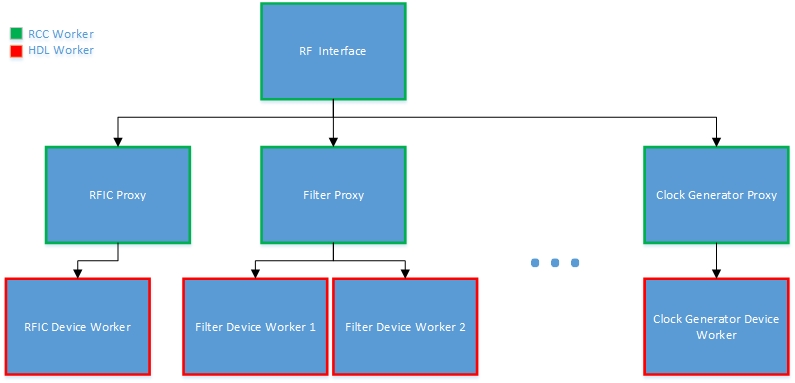
\includegraphics[scale=0.75]{figures/Generic_FE_diagram.jpg}
	\end{figure}
\newpage
\section{Control Interface}
Each setting has a max, min, and step value associated with it.  Where the max is the highest possible value, min is the lowest possible value, and step is the minimum granularity for changes of the associated setting.  These associated properties are available to be used by application developers for reading back information about the functionality of the interface during runtime.  Both receive and transmit use different spec files but have the same property sets. The component specification file locations are as follows: \\ \\
   \begin{tabular}{|p{2cm}|p{7cm}|}
      \hline
      Receive & core/specs/rx\_spec.xml \\
      \hline
      Transmit & core/specs/tx\_spec.xml  \\
      \hline
   \end{tabular}
   \\ \medskip \\
The properties that are described in these spec files can be observed in the following table.  For more details on these properties check the matchstiq\_rx or matchstiq\_tx data sheets. \\ \\
   \begin{longtable}{|p{5cm}|p{12cm}|}
			\hline
			\rowcolor{blue}
			Name                                & Usage                                                                                      \\
			\hline
			\verb+rf_gain_dB+                   & The runtime-configurable value in dB of the RF gain stage of the front-end receiver.        \\
			\hline
			\verb+rf_gain_max_dB+               & Maximum valid value for RF gain setting in dB. This value represents the datasheet-specified hardware limitations of the front-end's receiver, and therefore is buildtime-configurable only (i.e. it is a parameter). This property is intended to prevent the worker from re-configuring at runtime the RF amplifiers to have an invalid gain value. \\
			\hline
			\verb+rf_gain_min_dB+               & Minimum valid value for RF gain setting in dB. This value represents the datasheet-specified hardware limitations of the front-end's receiver, and therefore is buildtime-configurable only (i.e. it is a parameter). This property is intended to prevent the worker from re-configuring at runtime the RF amplifiers to have an invalid gain value. \\
			\hline
			\verb+rf_gain_step_dB+              & Minimum granularity for the RF gain setting in dB. This value represents the datasheet-specified hardware limitations of the front-end's receiver, and therefore is buildtime-configurable only (i.e. it is a parameter). This property serves two purposes: 1) to provide the end user with the knowledge of how the value applied to rf\_gain\_dB will be rounded, and 2) if necessary, to provide the worker implementation that is performing the rounding with the information necessary to do so. \\
			\hline
			\verb+bb_gain_dB+                   & The runtime-configurable value in dB of the baseband gain stage of the front-end receiver.  \\
			\hline
			\verb+bb_gain_max_dB+               & Maximum valid value for baseband gain setting in dB. This value represents the datasheet-specified hardware limitations of the front-end's receiver, and therefore is buildtime-configurable only (i.e. it is a parameter). This property is intended to prevent the worker from re-configuring at runtime the baseband amplifiers to have an invalid gain value. \\
			\hline
			\verb+bb_gain_min_dB+               & Minimum valid value for baseband gain setting in dB. This value represents the datasheet-specified hardware limitations of the front-end's receiver, and therefore is buildtime-configurable only (i.e. it is a parameter). This property is intended to prevent the worker from re-configuring at runtime the baseband amplifiers to have an invalid gain value. \\
			\hline
			\verb+bb_gain_step_dB+              & Minimum granularity for the baseband gain setting in dB. This value represents the datasheet-specified hardware limitations of the front-end's receiver, and therefore is buildtime-configurable only (i.e. it is a parameter). This property serves two purposes: 1) to provide the end user with the knowledge of how the value applied to bb\_gain\_dB will be rounded, and 2) if necessary, to provide the worker implementation that is performing the rounding with the information necessary to do so. \\
			\hline
			\verb+frequency_MHz+                & The runtime-configurable value in MHz for the tuned center frequency of the front-end receiver. \\
			\hline
			\verb+frequency_max_MHz+            & Maximum valid value for frequency setting in MHz. This value represents the datasheet-specified hardware limitations of the front-end's receiver, and therefore is buildtime-configurable only (i.e. it is a parameter). This property is intended to prevent the worker from re-configuring at runtime the front-end LO to have an invalid frequency value. \\
			\hline
			\verb+frequency_min_MHz+            & Minimum valid value for frequency setting in MHz. This value represents the datasheet-specified hardware limitations of the front-end's receiver, and therefore is buildtime-configurable only (i.e. it is a parameter). This property is intended to prevent the worker from re-configuring at runtime the front-end LO to have an invalid frequency value. \\
			\hline
			\verb+frequency_step_MHz+           & Minimum granularity for the frequency setting in MHz. This value represents the datasheet-specified hardware limitations of the front-end's receiver, and therefore is buildtime-configurable only (i.e. it is a parameter). This property serves two purposes: 1) to provide the end user with the knowledge of how the value applied to frequency\_MHz will be rounded, and 2) if necessary, to provide the worker implementation that is performing the rounding with the information necessary to do so. \\
			\hline
			\verb+sample_rate_MHz+              & The runtime-configurable sample rate of the front-end's ADC in MHz (MSps).                  \\
			\hline
			\verb+sample_rate_max_MHz+          & Maximum valid value for front-end ADC's sample rate setting in MHz (MSps). This value represents the datasheet-specified hardware limitations of the front-end's ADC, and therefore is buildtime-configurable only (i.e. it is a parameter). This property is intended to prevent the worker from re-configuring at runtime the ADC to have an invalid sample rate. \\
			\hline
			\verb+sample_rate_min_MHz+          & Minimum valid value for front-end ADC's sample rate setting in MHz (MSps). This value represents the datasheet-specified hardware limitations of the front-end's ADC, and therefore is buildtime-configurable only (i.e. it is a parameter). This property is intended to prevent the worker from re-configuring at runtime the ADC to have an invalid sample rate. \\
			\hline
			\verb+sample_rate_step_MHz+         & Minimum granularity for the ADC sample rate setting in MHz (MSps). This value represents the datasheet-specified hardware limitations of the front-end's ADC, and therefore is buildtime-configurable only (i.e. it is a parameter). This property serves two purposes: 1) to provide the end user with the knowledge of how the value applied to sample\_rate\_MHz will be rounded, and 2) to provide the worker implementation that is performing the rounding with the information necessary to do so. \\
			\hline
			\verb+rf_cutoff_frequency_MHz+      & The cutoff frequency in MHz for any filtering that is done in the RF stage of the front-end receiver. \\
			\hline
			\verb+rf_cutoff_frequency_max_MHz+  & Maximum valid value for RF cutoff frequency setting in MHz. This value represents the datasheet-specified hardware limitations of the front-end's receiver, and therefore is buildtime-configurable only (i.e. it is a parameter). This property is intended to prevent the worker from re-configuring at runtime the RF stage's filter(s) to have an invalid cutoff frequency. \\
			\hline
			\verb+rf_cutoff_frequency_min_MHz+  & Minimum valid value for RF cutoff frequency setting in MHz. This value represents the datasheet-specified hardware limitations of the front-end's receiver, and therefore is buildtime-configurable only (i.e. it is a parameter). This property is intended to prevent the worker from re-configuring at runtime the RF stage's filter(s) to have an invalid cutoff frequency. \\
			\hline
			\verb+rf_cutoff_frequency_step_MHz+ & Minimum granularity for the RF cutoff frequency setting in MHz. This value represents the datasheet-specified hardware limitations of the front-end's receiver, and therefore is buildtime-configurable only (i.e. it is a parameter). This property serves two purposes: 1) to provide the end user with the knowledge of how the value applied to rf\_cutoff\_frequency\_min\_MHz will be rounded, and 2) to provide the worker implementation that is performing the rounding with the information necessary to do so. \\
			\hline
			\verb+bb_cutoff_frequency_MHz+      & The cutoff frequency for any filtering that is done in the baseband stage of the front-end receiver. \\
			\hline
			\verb+bb_cutoff_frequency_max_MHz+  & Maximum valid value for baseband cutoff frequency in MHz. This value represents the datasheet-specified hardware limitations of the front-end's receiver, and therefore is buildtime-configurable only (i.e. it is a parameter). This property is intended to prevent the worker from re-configuring at runtime the baseband RF stage's filter(s) to have an invalid cutoff frequency. \\
			\hline
			\verb+bb_cutoff_frequency_min_MHz+  & Minimum valid value for baseband cutoff frequency in MHz. This value represents the datasheet-specified hardware limitations of the front-end's receiver, and therefore is buildtime-configurable only (i.e. it is a parameter). This property is intended to prevent the worker from re-configuring at runtime the baseband stage's filter(s) to have an invalid cutoff frequency. \\
			\hline
			\verb+bb_cutoff_frequency_step_MHz+ & Minimum granularity for the baseband cutoff frequency setting in MHz. This value represents the datasheet-specified hardware limitations of the front-end's receiver, and therefore is buildtime-configurable only (i.e. it is a parameter). This property serves two purposes: 1) to provide the end user with the knowledge of how the value applied to bb\_cutoff\_frequency\_min\_MHz will be rounded, and 2) to provide the worker implementation that is performing the rounding with the information necessary to do so. \\
			\hline
		\end{longtable}
\newpage
\section{Creating an Application using RF Interfaces}
As stated earlier, an application that uses an RF Interface Worker needs to also have any of the slave workers and slave of slave workers also declared in the application XML.  This may cause a different application XML per platform to declare the different dependencies per platform.  This is a limitation of the framework and will likely be fixed in a future release.  An example of how this will work is in both of the ANGRYVIPER Team's Reference applications: \\ \\
   \begin{tabular}{|p{2cm}|p{7cm}|}
      \hline
      FSK app & assets/applications/FSK \\
      \hline
      RX app & assets/applications/rx\_app  \\
      \hline
   \end{tabular}
   \\

\subsection{Application XML Example}
There are two ways that application developers can control the RF interface workers.  The first of which is to use the application XML with the ocpirun utility to set the properties as needed.  This is the easier of the two methods and works as long as the application doesn't need runtime-dynamic property control or user interaction to set initial properties.

\begin{verbatim}
<Application>
  <Instance component='ocpi.core.devices.rx'>
    <Property Name="bb_gain_dB"              Value="-5"/>
    <Property Name="rf_gain_dB"              Value="10"/>
    <Property Name="frequency_MHz"           Value="2400"/>
    <Property Name="sample_rate_MHz"         Value="5"/>
    <Property Name="bb_cutoff_frequency_MHz" Value="2.5"/>
    <Property Name="rf_cutoff_frequency_MHz" Value="2.5"/>
  </Instance>
  <Instance component='ocpi.core.devices.tx'>
    <Property Name="bb_gain_dB"              Value="-5"/>
    <Property Name="rf_gain_dB"              Value="10"/>
    <Property Name="frequency_MHz"           Value="2400"/>
    <Property Name="sample_rate_MHz"         Value="5"/>
    <Property Name="bb_cutoff_frequency_MHz" Value="2.5"/>
    <Property Name="rf_cutoff_frequency_MHz" Value="2.5"/>
  </Instance>

  ...

  The slaves of the RF interfaces and the slaves of the slaves

  ...

  The rest of the application and device workers required for the application

  ...

<Application>
\end{verbatim}

\newpage
\subsection{Application Control Interface Example}
The second way that an application developers can control the RF interface workers is via a C++ program that uses the Application Control Interface library which is provided with the OpenCPI framework.  This is required when the application user needs to interact with the application to change properties or if the properties of the workers need to change during a run of the application.

\begin{verbatim}
  ...
  setup application object
  ...

  double freq = 1000;
  app.getProperty("rx","frequency_min_MHz", value);
  double rx_frequency_min_MHz = atof(value.c_str());
  app.getProperty("rx","frequency_max_MHz", value);
  double rx_frequency_max_MHz = atof(value.c_str());
  if (bb_bw < rx_frequency_min_MHz || freq > rx_frequency_max_MHz)
  {
     printf("Error: invalid freq. setting to a default value. value: %f min: %f max: %f\n",
             freq, rx_frequency_min_MHz, rx_frequency_max_MHz);
     app.setProperty("rx","frequency_MHz", "2400");
  }

  ...
  start application or make other decisions based on settings passed in
  ...
\end{verbatim}
\newpage
\section{Implementation of a RF Interface Worker}

BSP Developers will need to add implementations of these RF interfaces when you want to add a new radio or RFIC card.  This section gives a brief walkthrough of how this is done and how it is different then normal RCC worker development.  These RF interfaces are just RCC workers with a few caveats, the interface workers generally have the ability to set the properties of several other workers and don't have a run function.  \\ \\
The framework has the ability to have a one to one slave master relationship between workers but there is no defined way to have multiple slaves.  The way workers can access multiple slaves is by using the ACI to access application properties.  a worker has the ability to access the application object that it is a part of.  This object is then used to access any properties within the application, so there is a lot of freedom.
\begin{verbatim}
  OA::Application &app  = getApplication();
  app.setProperty("rf_rx_proxy", "lpf_bw_hz", "750000")
\end{verbatim}
In this code snippet the application object is provided using the getApplication call and it is used to set the lpf\_bw\_hz property of a rf\_rxproxy component to 750000 Hz.  If there is not a rf\_rx\_proxy component in the application this call will throw an exception and the application will crash.  \\ \\
The framework also has the ability to call functions in the worker code before or after its properties are written by the container.  This is done in the following way within the worker:
\begin{verbatim}
  OWD(can't be in OWS):
     <specproperty name='frequency_MHz' writesync='1' default='500'/>

  C++:
  RCCResult frequency_MHz_written()
  {
     ...
     do work based on the property change.
     ...

     return RCC_OK;
  }

\end{verbatim}The following workers are good examples of how to create RF Interface workers:  \\ \\
   \begin{tabular}{|p{2cm}|p{10cm}|}
      \hline
      matchstiq\_rx & assets/hdl/platforms/matchstiq/devices/matchstiq\_rx.rcc/ \\
      \hline
      matchstiq\_tx & assets/hdl/platforms/matchstiq/devices/matchstiq\_tx.rcc/  \\
      \hline
   \end{tabular}

\end{document}
